% Options for packages loaded elsewhere
\PassOptionsToPackage{unicode}{hyperref}
\PassOptionsToPackage{hyphens}{url}
\documentclass[
]{article}
\usepackage{xcolor}
\usepackage[margin=1in]{geometry}
\usepackage{amsmath,amssymb}
\setcounter{secnumdepth}{-\maxdimen} % remove section numbering
\usepackage{iftex}
\ifPDFTeX
  \usepackage[T1]{fontenc}
  \usepackage[utf8]{inputenc}
  \usepackage{textcomp} % provide euro and other symbols
\else % if luatex or xetex
  \usepackage{unicode-math} % this also loads fontspec
  \defaultfontfeatures{Scale=MatchLowercase}
  \defaultfontfeatures[\rmfamily]{Ligatures=TeX,Scale=1}
\fi
\usepackage{lmodern}
\ifPDFTeX\else
  % xetex/luatex font selection
\fi
% Use upquote if available, for straight quotes in verbatim environments
\IfFileExists{upquote.sty}{\usepackage{upquote}}{}
\IfFileExists{microtype.sty}{% use microtype if available
  \usepackage[]{microtype}
  \UseMicrotypeSet[protrusion]{basicmath} % disable protrusion for tt fonts
}{}
\makeatletter
\@ifundefined{KOMAClassName}{% if non-KOMA class
  \IfFileExists{parskip.sty}{%
    \usepackage{parskip}
  }{% else
    \setlength{\parindent}{0pt}
    \setlength{\parskip}{6pt plus 2pt minus 1pt}}
}{% if KOMA class
  \KOMAoptions{parskip=half}}
\makeatother
\usepackage{color}
\usepackage{fancyvrb}
\newcommand{\VerbBar}{|}
\newcommand{\VERB}{\Verb[commandchars=\\\{\}]}
\DefineVerbatimEnvironment{Highlighting}{Verbatim}{commandchars=\\\{\}}
% Add ',fontsize=\small' for more characters per line
\usepackage{framed}
\definecolor{shadecolor}{RGB}{248,248,248}
\newenvironment{Shaded}{\begin{snugshade}}{\end{snugshade}}
\newcommand{\AlertTok}[1]{\textcolor[rgb]{0.94,0.16,0.16}{#1}}
\newcommand{\AnnotationTok}[1]{\textcolor[rgb]{0.56,0.35,0.01}{\textbf{\textit{#1}}}}
\newcommand{\AttributeTok}[1]{\textcolor[rgb]{0.13,0.29,0.53}{#1}}
\newcommand{\BaseNTok}[1]{\textcolor[rgb]{0.00,0.00,0.81}{#1}}
\newcommand{\BuiltInTok}[1]{#1}
\newcommand{\CharTok}[1]{\textcolor[rgb]{0.31,0.60,0.02}{#1}}
\newcommand{\CommentTok}[1]{\textcolor[rgb]{0.56,0.35,0.01}{\textit{#1}}}
\newcommand{\CommentVarTok}[1]{\textcolor[rgb]{0.56,0.35,0.01}{\textbf{\textit{#1}}}}
\newcommand{\ConstantTok}[1]{\textcolor[rgb]{0.56,0.35,0.01}{#1}}
\newcommand{\ControlFlowTok}[1]{\textcolor[rgb]{0.13,0.29,0.53}{\textbf{#1}}}
\newcommand{\DataTypeTok}[1]{\textcolor[rgb]{0.13,0.29,0.53}{#1}}
\newcommand{\DecValTok}[1]{\textcolor[rgb]{0.00,0.00,0.81}{#1}}
\newcommand{\DocumentationTok}[1]{\textcolor[rgb]{0.56,0.35,0.01}{\textbf{\textit{#1}}}}
\newcommand{\ErrorTok}[1]{\textcolor[rgb]{0.64,0.00,0.00}{\textbf{#1}}}
\newcommand{\ExtensionTok}[1]{#1}
\newcommand{\FloatTok}[1]{\textcolor[rgb]{0.00,0.00,0.81}{#1}}
\newcommand{\FunctionTok}[1]{\textcolor[rgb]{0.13,0.29,0.53}{\textbf{#1}}}
\newcommand{\ImportTok}[1]{#1}
\newcommand{\InformationTok}[1]{\textcolor[rgb]{0.56,0.35,0.01}{\textbf{\textit{#1}}}}
\newcommand{\KeywordTok}[1]{\textcolor[rgb]{0.13,0.29,0.53}{\textbf{#1}}}
\newcommand{\NormalTok}[1]{#1}
\newcommand{\OperatorTok}[1]{\textcolor[rgb]{0.81,0.36,0.00}{\textbf{#1}}}
\newcommand{\OtherTok}[1]{\textcolor[rgb]{0.56,0.35,0.01}{#1}}
\newcommand{\PreprocessorTok}[1]{\textcolor[rgb]{0.56,0.35,0.01}{\textit{#1}}}
\newcommand{\RegionMarkerTok}[1]{#1}
\newcommand{\SpecialCharTok}[1]{\textcolor[rgb]{0.81,0.36,0.00}{\textbf{#1}}}
\newcommand{\SpecialStringTok}[1]{\textcolor[rgb]{0.31,0.60,0.02}{#1}}
\newcommand{\StringTok}[1]{\textcolor[rgb]{0.31,0.60,0.02}{#1}}
\newcommand{\VariableTok}[1]{\textcolor[rgb]{0.00,0.00,0.00}{#1}}
\newcommand{\VerbatimStringTok}[1]{\textcolor[rgb]{0.31,0.60,0.02}{#1}}
\newcommand{\WarningTok}[1]{\textcolor[rgb]{0.56,0.35,0.01}{\textbf{\textit{#1}}}}
\usepackage{graphicx}
\makeatletter
\newsavebox\pandoc@box
\newcommand*\pandocbounded[1]{% scales image to fit in text height/width
  \sbox\pandoc@box{#1}%
  \Gscale@div\@tempa{\textheight}{\dimexpr\ht\pandoc@box+\dp\pandoc@box\relax}%
  \Gscale@div\@tempb{\linewidth}{\wd\pandoc@box}%
  \ifdim\@tempb\p@<\@tempa\p@\let\@tempa\@tempb\fi% select the smaller of both
  \ifdim\@tempa\p@<\p@\scalebox{\@tempa}{\usebox\pandoc@box}%
  \else\usebox{\pandoc@box}%
  \fi%
}
% Set default figure placement to htbp
\def\fps@figure{htbp}
\makeatother
\setlength{\emergencystretch}{3em} % prevent overfull lines
\providecommand{\tightlist}{%
  \setlength{\itemsep}{0pt}\setlength{\parskip}{0pt}}
\usepackage{bookmark}
\IfFileExists{xurl.sty}{\usepackage{xurl}}{} % add URL line breaks if available
\urlstyle{same}
\hypersetup{
  pdftitle={03\_clustering},
  pdfauthor={Anish},
  hidelinks,
  pdfcreator={LaTeX via pandoc}}

\title{03\_clustering}
\author{Anish}
\date{2026-04-26}

\begin{document}
\maketitle

\section{1. Goal of this notebook}\label{goal-of-this-notebook}

\section{2. Load PC scores and the original feature
table}\label{load-pc-scores-and-the-original-feature-table}

\begin{Shaded}
\begin{Highlighting}[]
\NormalTok{pc }\OtherTok{\textless{}{-}} \FunctionTok{read\_csv}\NormalTok{(}\StringTok{"../data/customer\_pc\_scores.csv"}\NormalTok{,}
               \AttributeTok{show\_col\_types =} \ConstantTok{FALSE}\NormalTok{)}
\NormalTok{customer }\OtherTok{\textless{}{-}} \FunctionTok{read\_csv}\NormalTok{(}\StringTok{"../data/customer\_features.csv"}\NormalTok{,}
                     \AttributeTok{show\_col\_types =} \ConstantTok{FALSE}\NormalTok{)}

\FunctionTok{dim}\NormalTok{(pc)}
\end{Highlighting}
\end{Shaded}

\begin{verbatim}
## [1] 4334    4
\end{verbatim}

\begin{Shaded}
\begin{Highlighting}[]
\FunctionTok{glimpse}\NormalTok{(pc)}
\end{Highlighting}
\end{Shaded}

\begin{verbatim}
## Rows: 4,334
## Columns: 4
## $ CustomerId <dbl> 12346, 12347, 12348, 12349, 12350, 12352, 12353, 12354, 123~
## $ PC1        <dbl> 1.3128225, 3.3557929, 0.7407239, 0.4667656, -1.9501216, 1.3~
## $ PC2        <dbl> -7.19782254, 0.17915017, 0.04036116, -2.12306976, -0.652095~
## $ PC3        <dbl> -2.8058725, 0.1402689, -0.1212519, -0.9784071, -0.5965301, ~
\end{verbatim}

\begin{Shaded}
\begin{Highlighting}[]
\CommentTok{\# Modelling matrix}
\NormalTok{Xpc }\OtherTok{\textless{}{-}}\NormalTok{ pc }\SpecialCharTok{|\textgreater{}} \FunctionTok{select}\NormalTok{(}\FunctionTok{starts\_with}\NormalTok{(}\StringTok{"PC"}\NormalTok{)) }\SpecialCharTok{|\textgreater{}} \FunctionTok{as.matrix}\NormalTok{()}
\FunctionTok{rownames}\NormalTok{(Xpc) }\OtherTok{\textless{}{-}}\NormalTok{ pc}\SpecialCharTok{$}\NormalTok{CustomerId}
\NormalTok{n\_pc }\OtherTok{\textless{}{-}} \FunctionTok{ncol}\NormalTok{(Xpc)}
\FunctionTok{sprintf}\NormalTok{(}\StringTok{"Clustering on \%d PCs across \%d customers"}\NormalTok{, n\_pc, }\FunctionTok{nrow}\NormalTok{(Xpc))}
\end{Highlighting}
\end{Shaded}

\begin{verbatim}
## [1] "Clustering on 3 PCs across 4334 customers"
\end{verbatim}

\section{3. K-means}\label{k-means}

\subsection{3a. Choosing K - WCSS /
elbow}\label{a.-choosing-k---wcss-elbow}

\begin{Shaded}
\begin{Highlighting}[]
\NormalTok{k\_grid }\OtherTok{\textless{}{-}} \DecValTok{2}\SpecialCharTok{:}\DecValTok{10}
\NormalTok{wcss }\OtherTok{\textless{}{-}} \FunctionTok{map\_dbl}\NormalTok{(k\_grid,}
\NormalTok{                \textbackslash{}(k) }\FunctionTok{kmeans}\NormalTok{(Xpc, }\AttributeTok{centers =}\NormalTok{ k, }\AttributeTok{nstart =} \DecValTok{25}\NormalTok{,}
                            \AttributeTok{iter.max =} \DecValTok{50}\NormalTok{)}\SpecialCharTok{$}\NormalTok{tot.withinss)}

\NormalTok{elbow\_df }\OtherTok{\textless{}{-}} \FunctionTok{tibble}\NormalTok{(}\AttributeTok{k =}\NormalTok{ k\_grid, }\AttributeTok{wcss =}\NormalTok{ wcss)}

\FunctionTok{ggplot}\NormalTok{(elbow\_df, }\FunctionTok{aes}\NormalTok{(k, wcss)) }\SpecialCharTok{+}
  \FunctionTok{geom\_line}\NormalTok{(}\AttributeTok{colour =} \StringTok{"steelblue"}\NormalTok{, }\AttributeTok{linewidth =} \DecValTok{1}\NormalTok{) }\SpecialCharTok{+}
  \FunctionTok{geom\_point}\NormalTok{(}\AttributeTok{colour =} \StringTok{"steelblue"}\NormalTok{, }\AttributeTok{size =} \DecValTok{2}\NormalTok{) }\SpecialCharTok{+}
  \FunctionTok{scale\_x\_continuous}\NormalTok{(}\AttributeTok{breaks =}\NormalTok{ k\_grid) }\SpecialCharTok{+}
  \FunctionTok{labs}\NormalTok{(}\AttributeTok{title =} \StringTok{"K{-}means: within{-}cluster sum of squares vs k"}\NormalTok{,}
       \AttributeTok{subtitle =} \StringTok{"Look for the kink — the elbow"}\NormalTok{,}
       \AttributeTok{x =} \StringTok{"k"}\NormalTok{, }\AttributeTok{y =} \StringTok{"Total WCSS"}\NormalTok{)}
\end{Highlighting}
\end{Shaded}

\pandocbounded{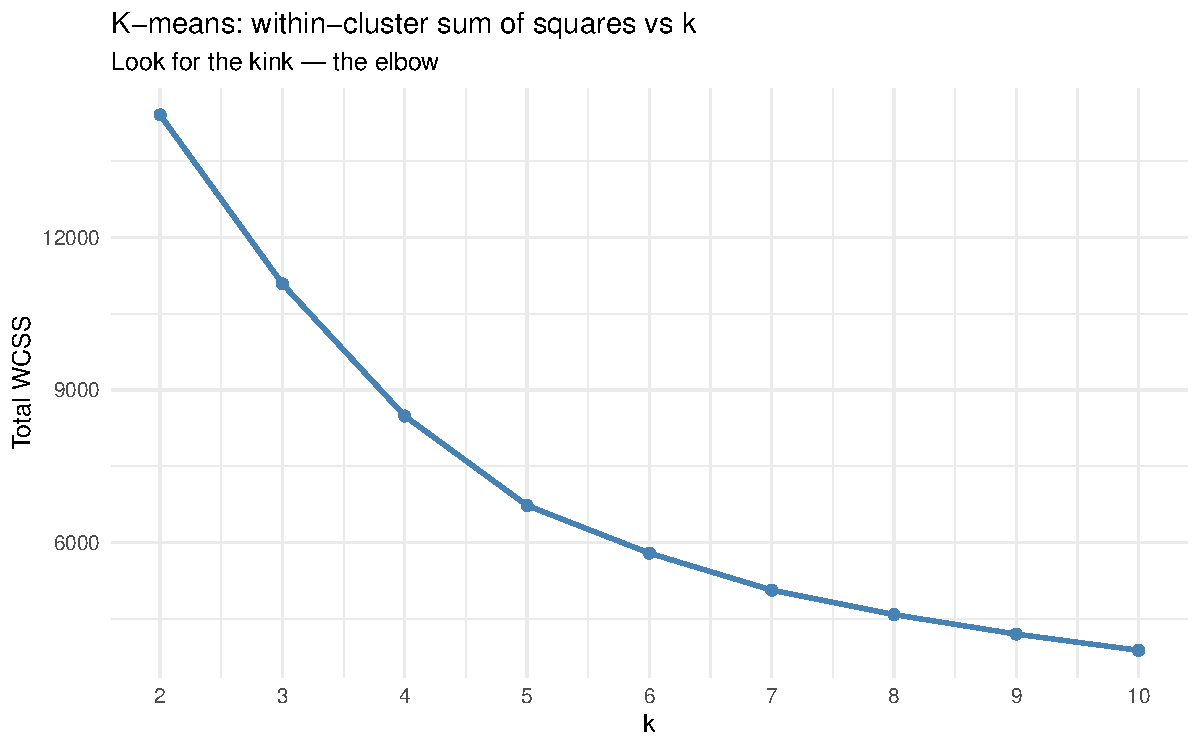
\includegraphics[keepaspectratio]{03_clustering_files/03_clustering_files/figure-latex/km-elbow-1.pdf}}

\subsection{3b. Silhouette width}\label{b.-silhouette-width}

\begin{Shaded}
\begin{Highlighting}[]
\NormalTok{d }\OtherTok{\textless{}{-}} \FunctionTok{dist}\NormalTok{(Xpc)   }\CommentTok{\# used by silhouette and hclust below}
\NormalTok{sil }\OtherTok{\textless{}{-}} \FunctionTok{map\_dbl}\NormalTok{(k\_grid, \textbackslash{}(k) \{}
\NormalTok{  cl }\OtherTok{\textless{}{-}} \FunctionTok{kmeans}\NormalTok{(Xpc, }\AttributeTok{centers =}\NormalTok{ k, }\AttributeTok{nstart =} \DecValTok{25}\NormalTok{, }\AttributeTok{iter.max =} \DecValTok{50}\NormalTok{)}\SpecialCharTok{$}\NormalTok{cluster}
  \FunctionTok{mean}\NormalTok{(}\FunctionTok{silhouette}\NormalTok{(cl, d)[, }\StringTok{"sil\_width"}\NormalTok{])}
\NormalTok{\})}
\NormalTok{sil\_df }\OtherTok{\textless{}{-}} \FunctionTok{tibble}\NormalTok{(}\AttributeTok{k =}\NormalTok{ k\_grid, }\AttributeTok{silhouette =}\NormalTok{ sil)}

\FunctionTok{ggplot}\NormalTok{(sil\_df, }\FunctionTok{aes}\NormalTok{(k, silhouette)) }\SpecialCharTok{+}
  \FunctionTok{geom\_line}\NormalTok{(}\AttributeTok{colour =} \StringTok{"darkorange"}\NormalTok{, }\AttributeTok{linewidth =} \DecValTok{1}\NormalTok{) }\SpecialCharTok{+}
  \FunctionTok{geom\_point}\NormalTok{(}\AttributeTok{colour =} \StringTok{"darkorange"}\NormalTok{, }\AttributeTok{size =} \DecValTok{2}\NormalTok{) }\SpecialCharTok{+}
  \FunctionTok{scale\_x\_continuous}\NormalTok{(}\AttributeTok{breaks =}\NormalTok{ k\_grid) }\SpecialCharTok{+}
  \FunctionTok{labs}\NormalTok{(}\AttributeTok{title =} \StringTok{"K{-}means: average silhouette width vs k"}\NormalTok{,}
       \AttributeTok{subtitle =} \StringTok{"Higher = more honest separation; pick the peak"}\NormalTok{,}
       \AttributeTok{x =} \StringTok{"k"}\NormalTok{, }\AttributeTok{y =} \StringTok{"Mean silhouette"}\NormalTok{)}
\end{Highlighting}
\end{Shaded}

\pandocbounded{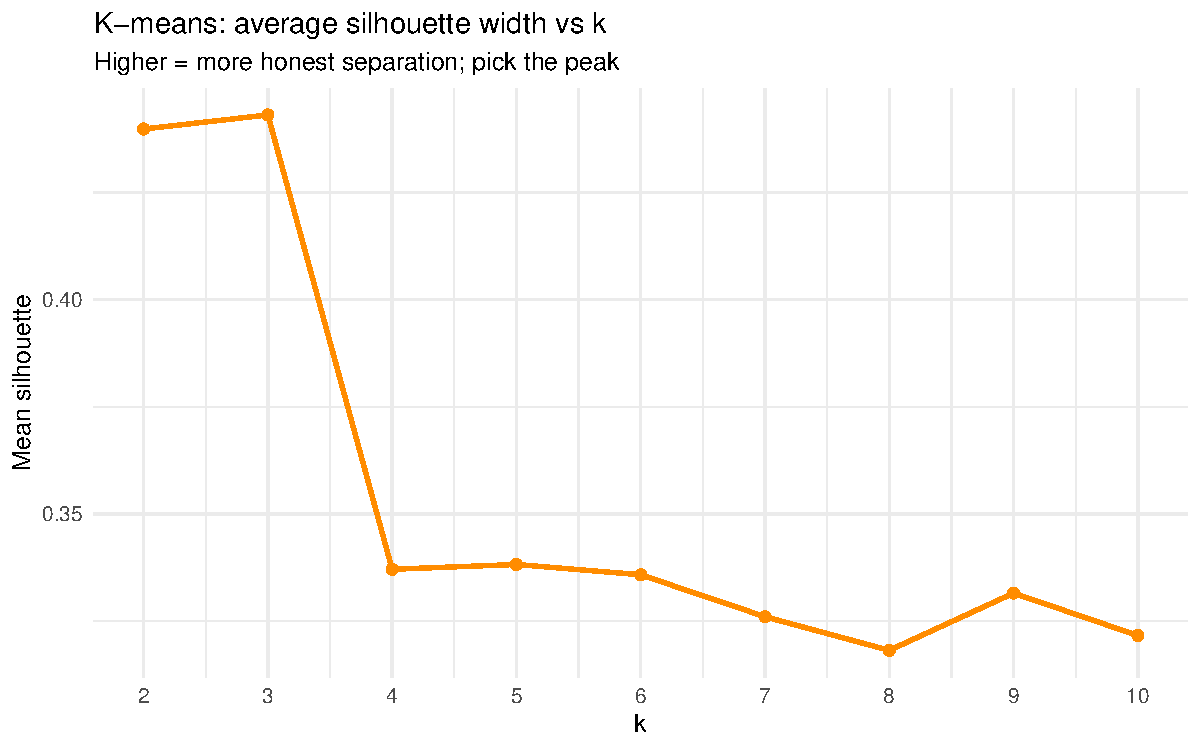
\includegraphics[keepaspectratio]{03_clustering_files/03_clustering_files/figure-latex/km-sil-1.pdf}}

\subsection{3c. Gap statistic}\label{c.-gap-statistic}

The most rigorous of the three (compares within-cluster dispersion to a
uniform-noise reference). Slow --- bumping \texttt{B} up gives smoother
estimates at the cost of runtime.

\begin{Shaded}
\begin{Highlighting}[]
\NormalTok{gap }\OtherTok{\textless{}{-}} \FunctionTok{clusGap}\NormalTok{(Xpc, }\AttributeTok{FUN =}\NormalTok{ kmeans, }\AttributeTok{nstart =} \DecValTok{25}\NormalTok{,}
               \AttributeTok{K.max =} \DecValTok{10}\NormalTok{, }\AttributeTok{B =} \DecValTok{50}\NormalTok{)}
\FunctionTok{print}\NormalTok{(gap, }\AttributeTok{method =} \StringTok{"Tibs2001SEmax"}\NormalTok{)}
\end{Highlighting}
\end{Shaded}

\begin{verbatim}
## Clustering Gap statistic ["clusGap"] from call:
## clusGap(x = Xpc, FUNcluster = kmeans, K.max = 10, B = 50, nstart = 25)
## B=50 simulated reference sets, k = 1..10; spaceH0="scaledPCA"
##  --> Number of clusters (method 'Tibs2001SEmax', SE.factor=1): 3
##           logW    E.logW      gap      SE.sim
##  [1,] 8.008122 10.013376 2.005254 0.005031357
##  [2,] 7.656533  9.695415 2.038883 0.004767524
##  [3,] 7.510463  9.557023 2.046560 0.004187232
##  [4,] 7.490680  9.423770 1.933090 0.003614868
##  [5,] 7.358716  9.330544 1.971828 0.002685959
##  [6,] 7.268588  9.251586 1.982998 0.002972993
##  [7,] 7.192272  9.206451 2.014180 0.002706496
##  [8,] 7.133030  9.164696 2.031666 0.002985710
##  [9,] 7.111730  9.127158 2.015428 0.003038975
## [10,] 7.031220  9.091784 2.060564 0.003282150
\end{verbatim}

\begin{Shaded}
\begin{Highlighting}[]
\FunctionTok{fviz\_gap\_stat}\NormalTok{(gap) }\SpecialCharTok{+}
  \FunctionTok{labs}\NormalTok{(}\AttributeTok{title =} \StringTok{"Gap statistic — Tibshirani 2001 SEmax rule"}\NormalTok{)}
\end{Highlighting}
\end{Shaded}

\pandocbounded{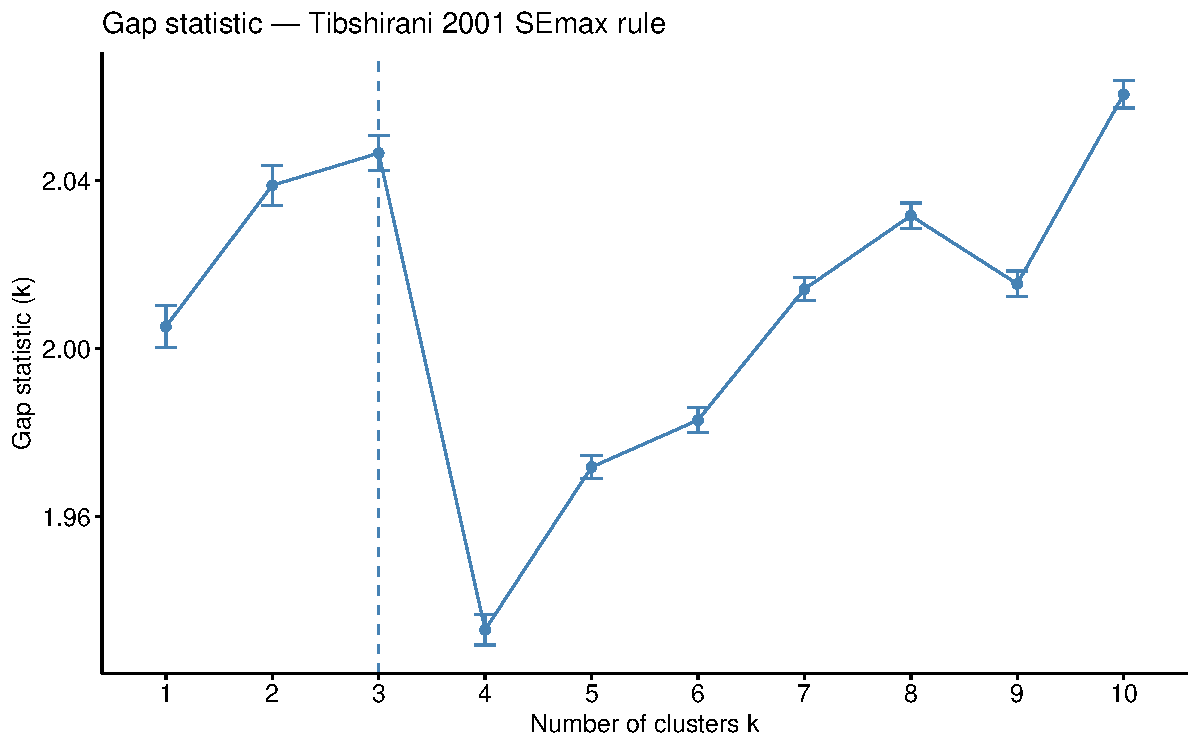
\includegraphics[keepaspectratio]{03_clustering_files/03_clustering_files/figure-latex/km-gap-1.pdf}}

\subsection{3d. Pick k and fit the final
model}\label{d.-pick-k-and-fit-the-final-model}

The three diagnostics often disagree by ±1. Pick the value that's
defensible under at least two and matches the substantive prior (4--6
clusters from the EDA discussion).

\begin{Shaded}
\begin{Highlighting}[]
\NormalTok{k\_star }\OtherTok{\textless{}{-}} \DecValTok{3}  \CommentTok{\# CHANGE if your diagnostics point elsewhere}

\NormalTok{km\_fit }\OtherTok{\textless{}{-}} \FunctionTok{kmeans}\NormalTok{(Xpc, }\AttributeTok{centers =}\NormalTok{ k\_star, }\AttributeTok{nstart =} \DecValTok{50}\NormalTok{, }\AttributeTok{iter.max =} \DecValTok{100}\NormalTok{)}
\NormalTok{km\_fit}\SpecialCharTok{$}\NormalTok{size                            }\CommentTok{\# cluster sizes}
\end{Highlighting}
\end{Shaded}

\begin{verbatim}
## [1] 1639 1487 1208
\end{verbatim}

\begin{Shaded}
\begin{Highlighting}[]
\FunctionTok{round}\NormalTok{(km\_fit}\SpecialCharTok{$}\NormalTok{centers, }\DecValTok{2}\NormalTok{)               }\CommentTok{\# centroids in PC space}
\end{Highlighting}
\end{Shaded}

\begin{verbatim}
##     PC1   PC2   PC3
## 1  0.01 -0.46 -0.24
## 2 -1.97  0.24  0.12
## 3  2.42  0.33  0.18
\end{verbatim}

\begin{Shaded}
\begin{Highlighting}[]
\FunctionTok{mean}\NormalTok{(}\FunctionTok{silhouette}\NormalTok{(km\_fit}\SpecialCharTok{$}\NormalTok{cluster, d)[, }\StringTok{"sil\_width"}\NormalTok{])}
\end{Highlighting}
\end{Shaded}

\begin{verbatim}
## [1] 0.3349896
\end{verbatim}

\section{4. Hierarchical clustering}\label{hierarchical-clustering}

\begin{itemize}
\tightlist
\item
  \textbf{Ward (\texttt{ward.D2})} --- minimises within-cluster
  variance, lines up philosophically with k-means. Usually the strongest
  single choice for customer segmentation.
\item
  \textbf{Complete} --- ISLR's default in the lab; tends to give
  compact, similar-diameter clusters.
\item
  \textbf{Average} --- friendlier to elongated or unequal-density
  clusters; used here as a robustness check.
\end{itemize}

\subsection{4a. Fit and plot
dendrograms}\label{a.-fit-and-plot-dendrograms}

\begin{Shaded}
\begin{Highlighting}[]
\NormalTok{hc\_ward     }\OtherTok{\textless{}{-}} \FunctionTok{hclust}\NormalTok{(d, }\AttributeTok{method =} \StringTok{"ward.D2"}\NormalTok{)}
\NormalTok{hc\_complete }\OtherTok{\textless{}{-}} \FunctionTok{hclust}\NormalTok{(d, }\AttributeTok{method =} \StringTok{"complete"}\NormalTok{)}
\NormalTok{hc\_average  }\OtherTok{\textless{}{-}} \FunctionTok{hclust}\NormalTok{(d, }\AttributeTok{method =} \StringTok{"average"}\NormalTok{)}
\end{Highlighting}
\end{Shaded}

\begin{Shaded}
\begin{Highlighting}[]
\FunctionTok{par}\NormalTok{(}\AttributeTok{mfrow =} \FunctionTok{c}\NormalTok{(}\DecValTok{3}\NormalTok{, }\DecValTok{1}\NormalTok{), }\AttributeTok{mar =} \FunctionTok{c}\NormalTok{(}\DecValTok{2}\NormalTok{, }\DecValTok{4}\NormalTok{, }\DecValTok{3}\NormalTok{, }\DecValTok{1}\NormalTok{))}
\FunctionTok{plot}\NormalTok{(hc\_ward,     }\AttributeTok{labels =} \ConstantTok{FALSE}\NormalTok{, }\AttributeTok{hang =} \SpecialCharTok{{-}}\DecValTok{1}\NormalTok{,}
     \AttributeTok{main =} \StringTok{"Ward (D2) linkage"}\NormalTok{,     }\AttributeTok{xlab =} \StringTok{""}\NormalTok{, }\AttributeTok{sub =} \StringTok{""}\NormalTok{)}
\FunctionTok{rect.hclust}\NormalTok{(hc\_ward, }\AttributeTok{k =}\NormalTok{ k\_star, }\AttributeTok{border =} \StringTok{"steelblue"}\NormalTok{)}

\FunctionTok{plot}\NormalTok{(hc\_complete, }\AttributeTok{labels =} \ConstantTok{FALSE}\NormalTok{, }\AttributeTok{hang =} \SpecialCharTok{{-}}\DecValTok{1}\NormalTok{,}
     \AttributeTok{main =} \StringTok{"Complete linkage"}\NormalTok{,      }\AttributeTok{xlab =} \StringTok{""}\NormalTok{, }\AttributeTok{sub =} \StringTok{""}\NormalTok{)}
\FunctionTok{rect.hclust}\NormalTok{(hc\_complete, }\AttributeTok{k =}\NormalTok{ k\_star, }\AttributeTok{border =} \StringTok{"darkorange"}\NormalTok{)}

\FunctionTok{plot}\NormalTok{(hc\_average,  }\AttributeTok{labels =} \ConstantTok{FALSE}\NormalTok{, }\AttributeTok{hang =} \SpecialCharTok{{-}}\DecValTok{1}\NormalTok{,}
     \AttributeTok{main =} \StringTok{"Average linkage"}\NormalTok{,       }\AttributeTok{xlab =} \StringTok{""}\NormalTok{, }\AttributeTok{sub =} \StringTok{""}\NormalTok{)}
\FunctionTok{rect.hclust}\NormalTok{(hc\_average,  }\AttributeTok{k =}\NormalTok{ k\_star, }\AttributeTok{border =} \StringTok{"firebrick"}\NormalTok{)}
\end{Highlighting}
\end{Shaded}

\pandocbounded{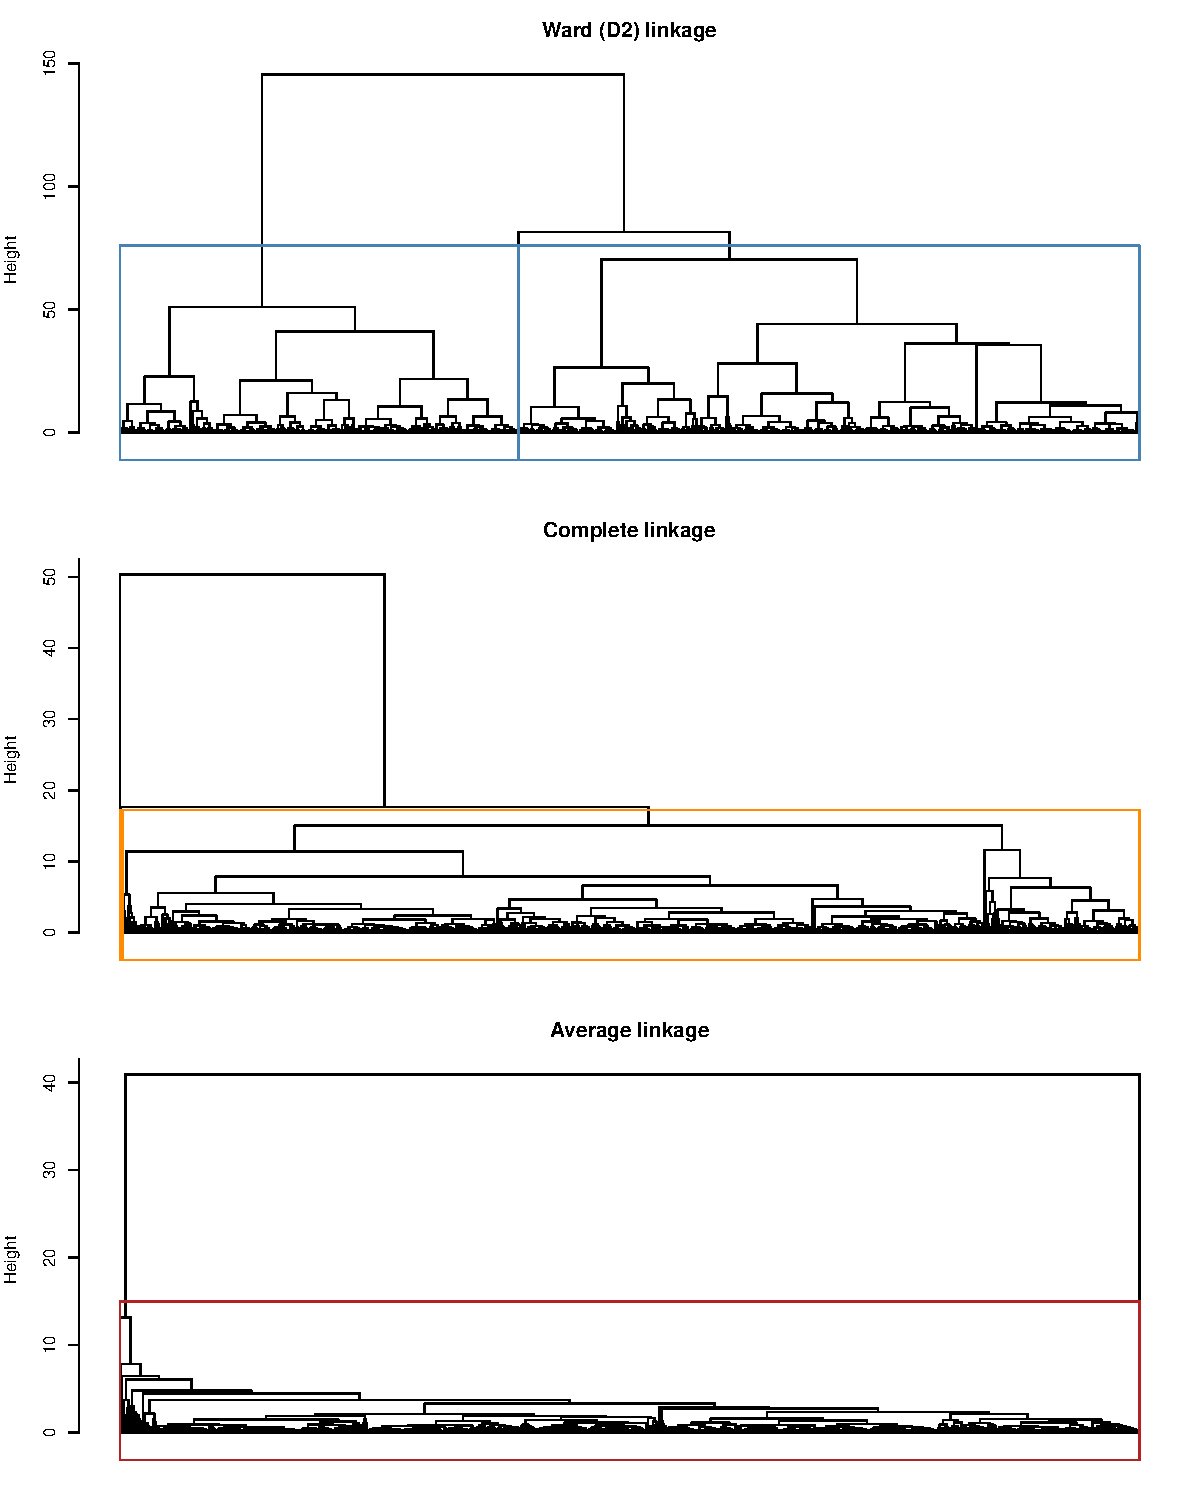
\includegraphics[keepaspectratio]{03_clustering_files/03_clustering_files/figure-latex/hc-dendrograms-1.pdf}}

\begin{Shaded}
\begin{Highlighting}[]
\FunctionTok{par}\NormalTok{(}\AttributeTok{mfrow =} \FunctionTok{c}\NormalTok{(}\DecValTok{1}\NormalTok{, }\DecValTok{1}\NormalTok{))}
\end{Highlighting}
\end{Shaded}

The dendrogram tells you whether \texttt{k\_star} is being forced or
whether the tree naturally falls into that many clusters. Ward and
complete should look broadly similar; if average linkage produces one
giant cluster and a handful of singletons, it's flagging a chaining
problem (a real concern with retail data) --- that's a finding, not a
bug.

\subsection{4b. Cut the tree at k* and compare to
k-means}\label{b.-cut-the-tree-at-k-and-compare-to-k-means}

\begin{Shaded}
\begin{Highlighting}[]
\NormalTok{hc\_cluster }\OtherTok{\textless{}{-}} \FunctionTok{cutree}\NormalTok{(hc\_ward, }\AttributeTok{k =}\NormalTok{ k\_star)}

\FunctionTok{table}\NormalTok{(}\AttributeTok{kmeans =}\NormalTok{ km\_fit}\SpecialCharTok{$}\NormalTok{cluster, }\AttributeTok{hclust =}\NormalTok{ hc\_cluster)}
\end{Highlighting}
\end{Shaded}

\begin{verbatim}
##       hclust
## kmeans    1    2    3
##      1 1152  486    1
##      2 1484    2    1
##      3    2 1206    0
\end{verbatim}

A nearly block-diagonal cross-tab means the two algorithms agree on
who's in which segment (just with different label numbers). Heavy
off-diagonal mass means the algorithms disagree about cluster boundaries
--- usually because k-means prefers spherical, equal-size clusters and
hierarchical doesn't.

\begin{Shaded}
\begin{Highlighting}[]
\FunctionTok{mean}\NormalTok{(}\FunctionTok{silhouette}\NormalTok{(hc\_cluster, d)[, }\StringTok{"sil\_width"}\NormalTok{])}
\end{Highlighting}
\end{Shaded}

\begin{verbatim}
## [1] 0.4323457
\end{verbatim}

\section{5. Stability --- bootstrap
Jaccard}\label{stability-bootstrap-jaccard}

This is the validation step that separates ``real structure'' from
``k-means happened to land somewhere.'' Resample customers (with
replacement), refit the clusterer, and measure how often the
\emph{original} clusters reappear. Jaccard ≥ 0.75 = ``stable cluster'',
\textless{} 0.6 = ``probably noise'' (Hennig 2007).

\begin{Shaded}
\begin{Highlighting}[]
\NormalTok{boot\_km }\OtherTok{\textless{}{-}} \FunctionTok{clusterboot}\NormalTok{(}
\NormalTok{  Xpc,}
  \AttributeTok{B            =} \DecValTok{50}\NormalTok{,}
  \AttributeTok{bootmethod   =} \StringTok{"boot"}\NormalTok{,}
  \AttributeTok{clustermethod =}\NormalTok{ kmeansCBI,}
  \AttributeTok{krange       =}\NormalTok{ k\_star,}
  \AttributeTok{seed         =} \DecValTok{1}\NormalTok{,}
  \AttributeTok{count        =} \ConstantTok{FALSE}
\NormalTok{)}
\FunctionTok{round}\NormalTok{(boot\_km}\SpecialCharTok{$}\NormalTok{bootmean, }\DecValTok{3}\NormalTok{)            }\CommentTok{\# one Jaccard per cluster}
\end{Highlighting}
\end{Shaded}

\begin{verbatim}
## [1] 0.878 0.926 0.921
\end{verbatim}

\begin{Shaded}
\begin{Highlighting}[]
\NormalTok{boot\_km}\SpecialCharTok{$}\NormalTok{bootbrd                        }\CommentTok{\# how often dissolved}
\end{Highlighting}
\end{Shaded}

\begin{verbatim}
## [1] 2 0 0
\end{verbatim}

\begin{Shaded}
\begin{Highlighting}[]
\NormalTok{boot\_hc }\OtherTok{\textless{}{-}} \FunctionTok{clusterboot}\NormalTok{(}
\NormalTok{  Xpc,}
  \AttributeTok{B            =} \DecValTok{50}\NormalTok{,}
  \AttributeTok{bootmethod   =} \StringTok{"boot"}\NormalTok{,}
  \AttributeTok{clustermethod =}\NormalTok{ hclustCBI,}
  \AttributeTok{method       =} \StringTok{"ward.D2"}\NormalTok{,}
  \AttributeTok{k            =}\NormalTok{ k\_star,}
  \AttributeTok{seed         =} \DecValTok{1}\NormalTok{,}
  \AttributeTok{count        =} \ConstantTok{FALSE}
\NormalTok{)}
\FunctionTok{round}\NormalTok{(boot\_hc}\SpecialCharTok{$}\NormalTok{bootmean, }\DecValTok{3}\NormalTok{)}
\end{Highlighting}
\end{Shaded}

\begin{verbatim}
## [1] 0.669 0.594 0.809
\end{verbatim}

\begin{Shaded}
\begin{Highlighting}[]
\NormalTok{boot\_hc}\SpecialCharTok{$}\NormalTok{bootbrd}
\end{Highlighting}
\end{Shaded}

\begin{verbatim}
## [1]  6 11 10
\end{verbatim}

\section{6. Visualise the final clusters in
PC1--PC2}\label{visualise-the-final-clusters-in-pc1pc2}

\begin{Shaded}
\begin{Highlighting}[]
\NormalTok{plot\_df }\OtherTok{\textless{}{-}}\NormalTok{ pc }\SpecialCharTok{|\textgreater{}}
  \FunctionTok{mutate}\NormalTok{(}\AttributeTok{km\_cluster =} \FunctionTok{factor}\NormalTok{(km\_fit}\SpecialCharTok{$}\NormalTok{cluster),}
         \AttributeTok{hc\_cluster =} \FunctionTok{factor}\NormalTok{(hc\_cluster))}

\FunctionTok{ggplot}\NormalTok{(plot\_df, }\FunctionTok{aes}\NormalTok{(PC1, PC2, }\AttributeTok{colour =}\NormalTok{ km\_cluster)) }\SpecialCharTok{+}
  \FunctionTok{geom\_point}\NormalTok{(}\AttributeTok{alpha =} \FloatTok{0.5}\NormalTok{, }\AttributeTok{size =} \FloatTok{0.8}\NormalTok{) }\SpecialCharTok{+}
  \FunctionTok{scale\_colour\_brewer}\NormalTok{(}\AttributeTok{palette =} \StringTok{"Set1"}\NormalTok{, }\AttributeTok{name =} \StringTok{"K{-}means"}\NormalTok{) }\SpecialCharTok{+}
  \FunctionTok{labs}\NormalTok{(}\AttributeTok{title =} \FunctionTok{sprintf}\NormalTok{(}\StringTok{"K{-}means clusters (k = \%d) in PC1–PC2"}\NormalTok{, k\_star))}
\end{Highlighting}
\end{Shaded}

\pandocbounded{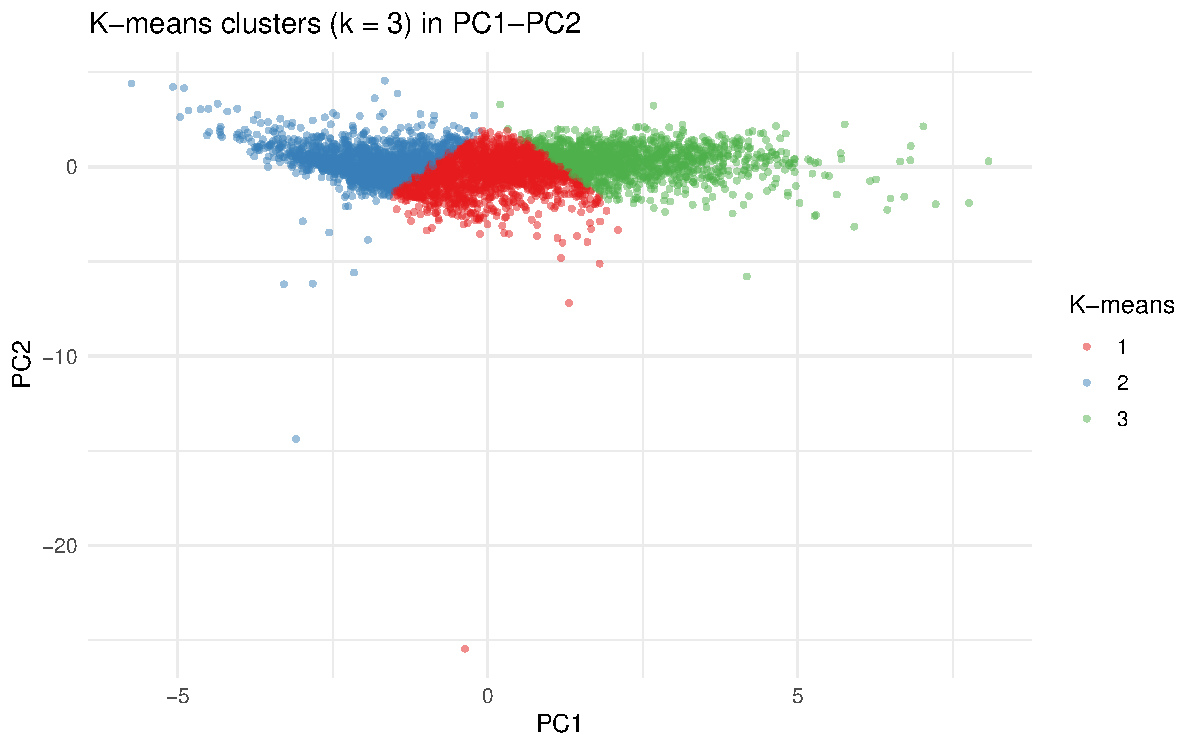
\includegraphics[keepaspectratio]{03_clustering_files/03_clustering_files/figure-latex/km-plot-1.pdf}}

\begin{Shaded}
\begin{Highlighting}[]
\FunctionTok{ggplot}\NormalTok{(plot\_df, }\FunctionTok{aes}\NormalTok{(PC1, PC2, }\AttributeTok{colour =}\NormalTok{ hc\_cluster)) }\SpecialCharTok{+}
  \FunctionTok{geom\_point}\NormalTok{(}\AttributeTok{alpha =} \FloatTok{0.5}\NormalTok{, }\AttributeTok{size =} \FloatTok{0.8}\NormalTok{) }\SpecialCharTok{+}
  \FunctionTok{scale\_colour\_brewer}\NormalTok{(}\AttributeTok{palette =} \StringTok{"Set2"}\NormalTok{, }\AttributeTok{name =} \StringTok{"Hierarchical (Ward)"}\NormalTok{) }\SpecialCharTok{+}
  \FunctionTok{labs}\NormalTok{(}\AttributeTok{title =} \FunctionTok{sprintf}\NormalTok{(}\StringTok{"Hierarchical clusters (Ward, k = \%d) in PC1–PC2"}\NormalTok{,}
\NormalTok{                       k\_star))}
\end{Highlighting}
\end{Shaded}

\pandocbounded{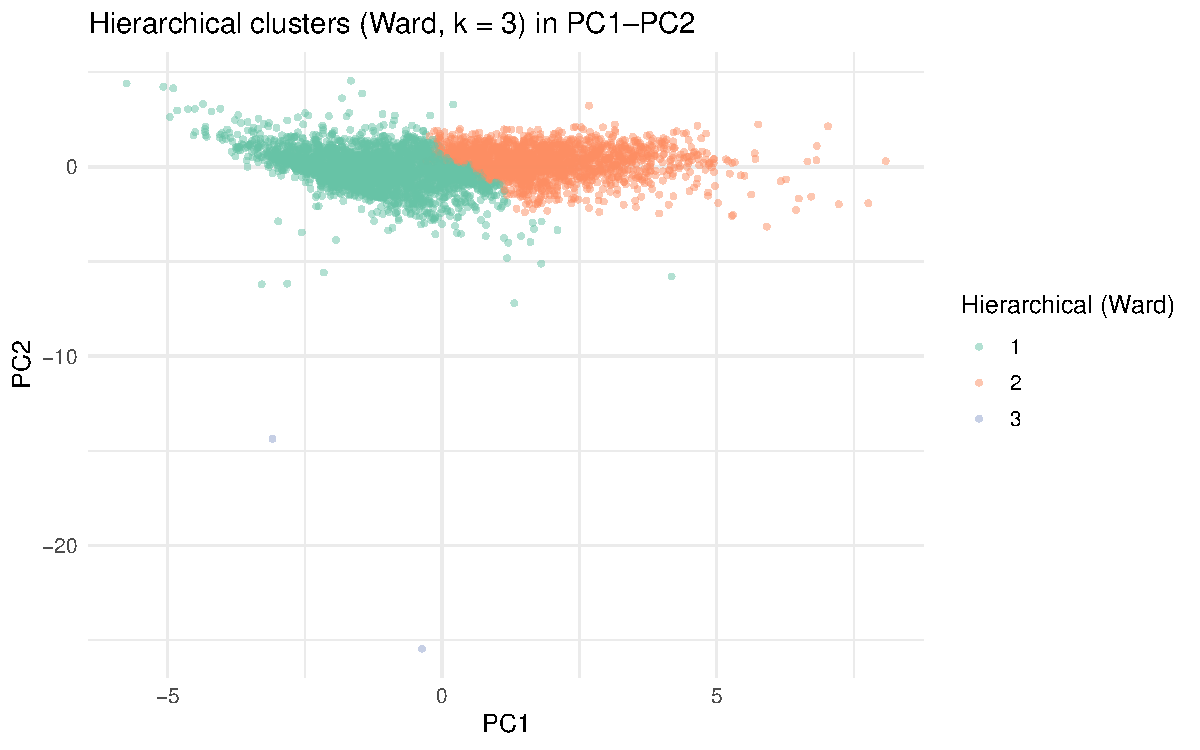
\includegraphics[keepaspectratio]{03_clustering_files/03_clustering_files/figure-latex/hc-plot-1.pdf}}

\begin{Shaded}
\begin{Highlighting}[]
\NormalTok{final\_label\_source }\OtherTok{\textless{}{-}} \StringTok{"kmeans"}   \CommentTok{\# CAN CHANGE to "hclust"}

\NormalTok{final\_cluster }\OtherTok{\textless{}{-}} \ControlFlowTok{if}\NormalTok{ (final\_label\_source }\SpecialCharTok{==} \StringTok{"kmeans"}\NormalTok{)}
\NormalTok{                   km\_fit}\SpecialCharTok{$}\NormalTok{cluster }\ControlFlowTok{else}\NormalTok{ hc\_cluster}

\NormalTok{assignments }\OtherTok{\textless{}{-}}\NormalTok{ pc }\SpecialCharTok{|\textgreater{}}
  \FunctionTok{select}\NormalTok{(CustomerId) }\SpecialCharTok{|\textgreater{}}
  \FunctionTok{mutate}\NormalTok{(}\AttributeTok{cluster        =} \FunctionTok{factor}\NormalTok{(final\_cluster),}
         \AttributeTok{cluster\_source =}\NormalTok{ final\_label\_source,}
         \AttributeTok{k              =}\NormalTok{ k\_star)}

\FunctionTok{write\_csv}\NormalTok{(assignments, }\StringTok{"../data/customer\_clusters.csv"}\NormalTok{)}

\NormalTok{assignments }\SpecialCharTok{|\textgreater{}} \FunctionTok{count}\NormalTok{(cluster, }\AttributeTok{name =} \StringTok{"customers"}\NormalTok{)}
\end{Highlighting}
\end{Shaded}

\begin{verbatim}
## # A tibble: 3 x 2
##   cluster customers
##   <fct>       <int>
## 1 1            1639
## 2 2            1487
## 3 3            1208
\end{verbatim}

\end{document}
